\section{Knapsack problems}

Informally, knapsack problems (KPs) may be described as finding the optimal combination of items from a set. Usually, this decision involves a certain value intrinsic to each item, and the objective is to maximize the total value of the selected items. To complicate this decision, items may have certain limiting values associated with them, which means not all of them may be selected.

The simplest example of a KP is the binary knapsack problem (BKP), also known as 0-1 knapsack problem \cite{ASSI2018}. It consists of a list of $n$ items, each with a value $v_i$ and a weight $w_i$ associated with them, for $i \in \{1,\dots,n\}$. A subset of items must be selected in order to maximize the total value, subject to a maximum weight capacity\footnote{This limiting factor, which can be interpreted as a bag or a container, is what gives the KP its name.} $C$. One may thus formulate the BKP as \cref{eq:ip:bkp},

\begin{align}
    \label[ip]{eq:ip:bkp}
    \begin{split}
        \max &\sum_{i=1}^{n}x_iv_i\\
        \textrm{s. t.}& \sum_{i=1}^{n}x_iw_i \leq C,\\
        &x_i \in \{0,1\} \quad \forall i \in \{1,\dots,n\},
    \end{split}
\end{align}
where $x_i$ are decision variables that specify whether item $i \in \{1,\dots,n\}$ has been selected or not.

By introducing slight variations to this formulation, it is possible to obtain many different uses for the KP:

\begin{itemize}
    \item Unbounded knapsack problem (UKP): By letting $x_i \in \mathbb{N}$, the number of units of each item available is unlimited.
    \item Fractional knapsack problem (FKP): By letting $x_i \in [0, 1]$, a fraction of each item can be selected.
    \item Subset sum problem (SSP): When $v_i = w_i \, \forall i \in \{1,\dots,n\}$, the objective can be interpreted as maximizing the weight of the knapsack. Furthermore, if we demand that $\sum_{i=1}^{n}x_iw_i = C$, then the problem becomes finding the combination of items that produces sum $C$ exactly \cite{FEOFILOFF2020b}.
\end{itemize}

The KP can be further complicated by taking into account multiple knapsacks and constraints. In this section, we focus on the latter.

\subsection{Simple algorithms for the binary knapsack problem}

The selection of subsets implies that an upper bound on the number of solutions to the BKP is $2^n$. Therefore, a natural first solution to the problem is a recursive binary tree algorithm \cite{FEOFILOFF2020a}. Let $I = \{1,\dots,n\}$ be the set of items to be put in the knapsack. Then, by representing the values and weights of items as entries in vectors $v, w \in \mathbb{R}^n$, respectively, and the remaining knapsack weight capacity as $c \in \mathbb{R}$, we arrive at \cref{alg:kp tree algorithm} for an instance $\phi(n, c, X, s)$ of the problem, where $X \subseteq I$ is the set of selected items and $s$ is the sum of said items' values at the node.

\begin{algorithm}
    \caption{\href{https://github.com/phcentenaro7/IC-Knapsack/blob/main/Knapsack/USP/recursive_knapsack.jl}{Recursive binary tree algorithm for the KP: $\phi(n, c, X, s)$}}
    \label{alg:kp tree algorithm}
    \begin{algorithmic}[1]
        \If{$n=0$} \label{alg:kp tree algorithm ln1}
            \State return $(X, s)$
        \EndIf
        \State $X_1, s_1 \coloneqq \phi(n - 1, c, X, s)$ \label{alg:kp tree algorithm ln2}
        \State $X_2, s_2 \gets (\emptyset, \emptyset)$
        \If{$w_n \leq c$}
            \State $X_2, s_2 \coloneqq \phi(n - 1, c - w_n, X \cup \{n\}, s + v_n)$
        \EndIf
        \State $s \coloneqq max(s_1, s_2)$ \label{alg:kp tree algorithm ln3}
        \State $X_3 \gets 0$
        \If{$v = v_1$}
            \State $X_3 \coloneqq X_1$
        \Else
            \State $X_3 \coloneqq X_2$
        \EndIf
        \State return $(X_3, s)$
    \end{algorithmic}
\end{algorithm}

The algorithm consists of a top-bottom phase, in which the nodes are generated, and a bottom-top phase, in which the optimal solution is found. The top-bottom phase begins at \cref{alg:kp tree algorithm ln2}, where a new instance of $\phi$ is called with item $n$ discarded from the solution. Subsequently, if there is enough capacity left in the knapsack, a second node is generated, with $n$ included in the solution.

When $n = 0$ (\cref{alg:kp tree algorithm ln1}), it is impossible to generate a new node. Thus, the only remaining action is to return the solution set at the node and its value sum. Once the whole tree has been generated, \cref{alg:kp tree algorithm ln3} is reached. From this point on, the bottom-top phase begins, with each node selecting the best solution its children have to offer. Hence, the optimal solution is returned by the root node.

Due to the combinatorial nature of the KP, \cref{alg:kp tree algorithm} is only efficient at solving small problems \cite{FEOFILOFF2020a}.

\begin{example}
    Suppose we have a knapsack with maximum capacity $C = 5$ and three items. The weight vector is $w = [1, 2, 3]$ and the value vector is $v = [2, 4, 3]$. By applying \cref{alg:kp tree algorithm} to this problem, we obtain the tree in \cref{fig:kp tree example}.

    \begin{figure}[h]
        \centering
        \begin{tikzpicture}[>=Stealth]
            \graph[binary tree layout]{
              l0n1[as=0] -> {
                l1n1[as=0] -> {
                    l2n1[as=0] -> {
                        l3n1[as=0],
                        l3n2[as=2]
                    },
                    l2n2[as=4] -> {
                        l3n3[as=4],
                        l3n4[as=6]
                    }
                },
                l1n2[as=3] -> {
                    l2n3[as=3] -> {
                        l3n5[as=3],
                        l3n6[as=5]
                    },
                    l2n4[as=7] -> l3n7[as=7]
                }
              }
            };
        \end{tikzpicture}
        \caption{BKP binary tree algorithm example.}
        \label{fig:kp tree example}
    \end{figure}
    Each node in the tree represents the value sum of a feasible combination of items. It immediately becomes clear that the optimal solution in this case is $7$, with the combination of items $2$ and $3$. However, this is not obvious to the computer, which must solve every recursion and return to the root node first.
\end{example}

Dynamic programming \cite{BRADLEY1977,WAGNER1995} approaches to the KP exist \cite{FEOFILOFF2020a,HRISTAKEVA2005,DEMAINE2011}. The idea behind these approaches is to generate a table with solutions to subproblems of the KP, using previous calculations to shorten the path to the optimal solution.

Let $T \in \mathbb{R}^{(n+1) \times (c+1)}$ be the dynamic programming table for the KP. \cref{alg:kp dynamic programming} exemplifies how $T$ can be constructed and used to arrive at the optimal KP solution.

\begin{algorithm}
    \caption{\href{https://github.com/phcentenaro7/IC-Knapsack/blob/main/Knapsack/USP/dynamic_knapsack.jl}{Dynamic programming algorithm for the KP: $\Phi(n, c)$}}
    \label{alg:kp dynamic programming}
    \begin{algorithmic}[1]
        \For{$i$ from $1$ to $n+1$} \label{dpln1}
            \State $T_{i,1} \coloneqq 0$
        \EndFor
        \For{$j$ from $2$ to $c+1$}
            \State $T_{1,j} \coloneqq 0$ \label{dpln2}
            \For{$i$ from $2$ to $n+1$} \label{dpln3}
                \State $T_{i,j} \gets T_{i-1,j}$
                \If{$w_i \leq j$}
                    \State $T_{i,j} \gets \max{(T_{i,j}, v_{i-1} + T_{i-1,j-w_{i-1}})}$\label{dpln4}
                \EndIf
            \EndFor
        \EndFor
        \State $n_i, c_i, X \gets (n, c, \emptyset)$
        \While{$c_i > 0$} \label{dpln5}
            \If{$T_{n_i+1, c_i+1} \neq T_{n_i, c_i+1}$}
                \State $X \gets X \cup n_i$
                \State $c_i \gets c_i - w_n$
            \EndIf
            \State $n_i \gets n_i - 1$
        \EndWhile
        \State return X
    \end{algorithmic}
\end{algorithm}

$T_{i,j}$ represents the optimal value for a subproblem of the KP with $i - 1$ items and knapsack capacity $j - 1$. Consequently, no set of items can satisfy $j = 1$, and so $T_{i,1} = 0 \, \forall i \in \{1,\dots,n + 1\}$. Furthermore, since there are no items to select when $i = 1$, it follows that $T_{1,j} = 0 \, \forall j \in \{1,\dots,c + 1\}$. This explains lines \ref{dpln1} through \ref{dpln2}.

Lines \ref{dpln3} through \ref{dpln4} fill the remaining entries in the table. If $w_{i-1} > j - 1$, we simply keep the best solution found so far for capacity $j - 1$. Otherwise, we compare said solution with what would be obtained if $i - 1$ was selected. The larger value becomes entry $T_{i,j}$.

Once table $T$ is finished, starting at \cref{dpln5}, the process of determining what items constitute an optimal solution occurs. Following the logic of lines \ref{dpln3} through \ref{dpln4}, if $T_{i,j} = T_{i-1,j}$, then the current item has not been selected and we may move on to the next item. Otherwise, the item is included in the final solution and we move on to the next item with less capacity, $T_{i-1,j-w_i}$.

Though better than the binary tree approach, the dynamic programming algorithm's complexity is exponential as well \cite{FEOFILOFF2020a}. In fact, this approach is notably inefficient for large capacity values \cite{HRISTAKEVA2005}.

\begin{example}
    Suppose the following problem suggested by \textcite{FEOFILOFF2020a}: We have $4$ items and a capacity $5$. The weights and values of items are, respectively, $w = [4, 2, 1, 3]$ and $v = [500, 400, 300, 450]$. To find the optimal solution to this BKP, we start by applying the part of \cref{alg:kp dynamic programming} to generate \cref{tab:kp dynamic programming table}.

    \begin{table}[h]
        \centering
        \begin{tabular}{|c c c c c c|}
            \hline
            0 & 0 & 0 & 0 & 0 & 0\\
            \hline
            0 & 0 & 0 & 0 & 500 & 500\\
            \hline
            0 & 0 & 400 & 400 & 500 & 500\\
            \hline
            0 & 300 & 400 & 700 & 700 & 800\\
            \hline
            0 & 300 & 400 & 700 & 750 & 850\\
            \hline
        \end{tabular}
        \caption{BKP dynamic programming table example.}
        \label{tab:kp dynamic programming table}
    \end{table}

    Next, we start looking for the solution from the table's bottom right entry. We note that $T_{5,6} \neq T_{4,6}$. This means that item $4 \in X$ (the solution set). Next, we investigate item $3$. Since $4 \in X$, that means the capacity is now at $5 - w_4 = 2$. So we look at $T_{4,3}$, which is equal to $T_{3,3}$. We conclude that $3 \notin X$. Moving up a row, $T_{3,3} \neq T_{2,3}$, which means $2 \in X$. By repeating this one more time, we conclude that $X = \{2,4\}$.
\end{example}

Along with these algorithms, an \href{https://github.com/phcentenaro7/IC-Knapsack/blob/main/Knapsack/Misc/1DKP.jl}{integer programming model} of the BKP was implemented in JuMP.

\subsection{Models for multidimensional knapsack problems}

Since the BKP contains a single capacity constraint (see \cref{eq:ip:bkp}), we can think of each item as a line segment whose length is $w_i$. It follows that the sum of lengths of the items must not exceed capacity $C$.

We wish to extrapolate this geometric interpretation of the BKP in a way that allows us to solve problems related to areas and volumes. In other words, we want to formulate two- and three-dimensional knapsack problems. To arrive at such formulations, first consider the multidimensional knapsack problem (MKP) \cite{LAABADI2018}, formulated in \cref{eq:ip:mkp}.

\begin{align}
    \label[ip]{eq:ip:mkp}
    \begin{split}
        \max & \sum_{i=1}^{n}v_ix_i\\
        \text{s. t.}& \sum_{i=1}^{n}w_{ji}x_i \leq C_j, \quad \forall j \in \{1,\dots,d\}\\
        & x_i \in \{0,1\}, \quad \forall i \in \{1,\dots,n\}.
    \end{split}
\end{align}

A number of differences can be spotted in this model, compared to the BKP's. The first is the introduction of parameter $d \in \mathbb{R}$, the number of dimensions that are being taken into account. Capacity $C \in \mathbb{R}$ becomes $C \in \mathbb{R}^d$, and each item $i \in \{1,\dots,n\}$ now has an associated vector $w_{ji} \in \mathbb{R}^{d}$ describing its weight across the problem's dimensions.

Specifically in the case of two dimensions, we may rewrite this formulation as \cref{eq:ip:mkp2d}.

\begin{align}
    \label[ip]{eq:ip:mkp2d}
    \begin{split}
        \max & \sum_{i=1}^{n}v_ix_i\\
        \text{s. t.}& \sum_{i=1}^{n}w_ix_i \leq W,\\
        & \sum_{i=1}^{n}h_ix_i \leq H,\\
        & x_i \in \{0,1\}, \quad \forall i \in \{1,\dots,n\}.
    \end{split}
\end{align}

Here, $w_i$ and $h_i$ represent the width and height of item $i$, while $W$ and $H$ represent the width and height of the container where we wish to place the items. We assume both the items and the container to be rectangular.

Suppose we want to place three items within a $30 \times 20$ container. The width, height and value vectors for this problem are $w = [10, 10, 5]$, $h = [5, 10, 15]$ and $v = [10, 15, 5]$. Through the plot on the left in \cref{fig:mkp2d example}, we can see that this is a trivial task. All items are selected and the optimal value is $30$.

Our MKP formulation begs to differ: Only items $1$ and $2$ are selected, for an optimal value of $25$. Why? The plot on the right illustrates the issue: The MKP is applying the line segment logic to multiple dimensions, as if each chosen subset of items ended up constituting a larger rectangle of dimensions $\sum_{i=1}^{n}w_i \times \sum_{i=1}^{n}h_i$.

\begin{figure}[h]
    \centering
    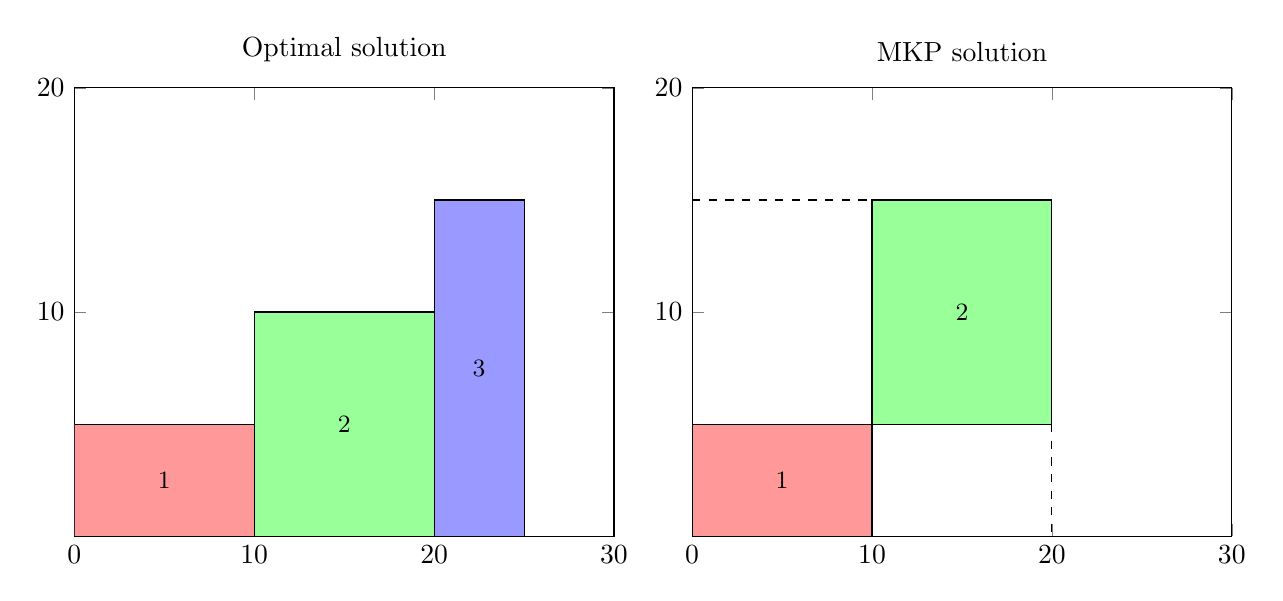
\begin{tikzpicture}
        % \begin{pgfonlayer}{background}
        %     \includegraphics[scale=0.3]{Hero-20Pedigree-20Cats_jpg.png}
        %  \end{pgfonlayer}
        \begin{axis}[title=Optimal solution, xmin=0, xmax=30, ymin=0, ymax=20, xtick={0, 10, 20, 30}, ytick={10, 20}, name=optimal]
            \filldraw [draw=black, fill=red!40] (axis cs:0,0) rectangle (axis cs:10, 5);
            \node [black] at (axis cs:5, 2.5){\small{1}};
            \filldraw [draw=black, fill=green!40] (axis cs:10, 0) rectangle (axis cs:20, 10);
            \node [black] at (axis cs:15, 5){\small{2}};
            \filldraw [draw=black, fill=blue!40] (axis cs:20, 0) rectangle (axis cs:25, 15);
            \node [black] at (axis cs:22.5, 7.5){\small{3}};
            \addplot [draw=none] coordinates{(0,0)};
        \end{axis}
        \begin{axis}[at=(optimal.right of east), anchor=west, title=MKP solution, xmin=0, xmax=30, ymin=0, ymax=20, xtick={0, 10, 20, 30}, ytick={10, 20}, name=wrong,  xshift=0.7cm]
            \filldraw [draw=black, fill=red!40] (axis cs:0,0) rectangle (axis cs:10, 5);
            \node [black] at (axis cs:5, 2.5){\small{1}};
            \filldraw [draw=black, fill=green!40] (axis cs:10, 5) rectangle (axis cs:20, 15);
            \node [black] at (axis cs:15, 10){\small{2}};
            \draw [dashed] (axis cs:0, 15) -- (axis cs:10, 15);
            \draw [dashed] (axis cs:20, 5) -- (axis cs:20, 0);
            \addplot [draw=none] coordinates{(0,0)};
        \end{axis}
    \end{tikzpicture}
    \caption{Bidimensional items within a $30 \times 20$ container.}
    \label{fig:mkp2d example}
\end{figure}

We need to sophisticate our model's constraints in order to solve 2D knapsack problems. We begin by introducing variables $x_i, y_i \in \mathbb{R}$, which describe the position of each item's bottom-left corner. It immediately becomes clear that every selected item $i \in \{1,\dots,n\}$ must obey \cref{eq:2DKP item corner constraints},

\begin{align}
    \label[constraint set]{eq:2DKP item corner constraints}
    \begin{split}
        0 \leq x_i \leq W,\\
        0 \leq x_i + w_i \leq W,\\
        0 \leq y_i \leq H,\\
        0 \leq y_i + h_i \leq H,
    \end{split}
\end{align}
where $W$ and $H$ are the width and height of the container, respectively.

Our task is complicated by the need to avoid item overlap. To accomplish this, we adopt the approach described by \textcite{KALVELAGEN2021}. For every selected item $i, j \in \{1,\dots,n\}$ with $i \neq j$, at least one inequality from \cref{eq:2DKP no-overlap intro} must hold true.

\begin{align}
    \label[constraint set]{eq:2DKP no-overlap intro}
    \begin{split}
        x_i + w_i \leq x_j,\\
        x_j + w_j \leq x_i,\\
        y_i + h_i \leq y_j,\\
        y_j + h_j \leq y_i.
    \end{split}
\end{align}

If we force all of these constraints upon the model, that might result in slower solve times. Thus, we need a way to enforce one constraint \emph{or} another. In other words, we have \emph{alternative constraints} \cite{BRADLEY1977}.

To implement this behavior in a 2DKP model, \textcite{KALVELAGEN2021} resorts to \emph{conditional constraints}, defined by \textcite{BRADLEY1977} as constraints of the form

\begin{equation}
    f_1(x_1,x_2,\dots,x_n) > b_1 \Rightarrow f_2(x_1,x_2,\dots,x_n) \leq b_2.
\end{equation}

In our case, the desired relations are given by variables $\delta_{i,j,k} \in \{0,1\}, \, k \in \{1,\dots,4\}$:

\begin{align}
    \delta_{i,j,1} = 1 \Rightarrow x_i + w_i \leq x_j,\\
    \delta_{i,j,2} = 1 \Rightarrow x_j + w_j \leq x_i,\\
    \delta_{i,j,3} = 1 \Rightarrow y_i + h_i \leq y_j,\\
    \delta_{i,j,4} = 1 \Rightarrow y_j + h_j \leq y_i.
\end{align}

These constraints can be mathematically implemented as \emph{big M constraints}\footnote{the concept is similar to the big M method for solving linear programming problems \cite{BAZARAA2010,BERTSIMAS1997}}. The idea is to introduce a constant $M \to +\infty$ and rewrite the constraints as

\begin{align}
    x_i + w_i - M(1 - \delta_{i,j,1}) \leq x_j,\\
    x_j + w_j - M(1 - \delta_{i,j,2}) \leq x_i,\\
    y_i + h_i - M(1 - \delta_{i,j,3}) \leq y_j,\\
    y_j + h_j - M(1 - \delta_{i,j,4}) \leq y_i.
\end{align}

Finally, we add the following constraint:

\begin{equation}
    \sum_{k=1}^{n} \delta_{i,j,k} \geq 1.
\end{equation}

For $M \to +\infty$, if a certain constraint is not selected, it's obvious that the inequations hold. This remains true for any item smaller than the container when $M = \max\{W,H\}$.

It is possible to introduce rotations to this model. For this purpose, we create new variables $\sigma_i$. When item $i$ is rotated, $\sigma_i = 1$. Otherwise, $\sigma_i = 0$. Then, the following constraints must be introduced:

\begin{align}
    x'_i = x_i + (1-\sigma_i)w_i + \sigma_i h_i,\\
    y'_i = y_i + (1-\sigma_i)h_i + \sigma_i w_i.
\end{align}

% If $(x_i, y_i)$ represents the bottom-left corner of an item, then $(x'_i, y'_i)$ represent the top-right corner adjusted for the correct rotation.

Having made all of these considerations, we can finally produce our continuous 2DKP model. Here, $s_i$ are the decision variables. For brevity, consider $N = \{1,\dots,n\}$.

\begin{subequations}
    \label[mip]{eq:ip:2DKP continuous}
    \begin{align}
        \max&\sum_{i \in N}v_i s_i\\
        \text{s. t.}& 0 \leq x_i \leq W, \quad \forall i \in N,\\
        & 0 \leq x'_i \leq W, \quad \forall i \in N,\\
        & 0 \leq y_i \leq H, \quad \forall i \in N,\\
        & 0 \leq y'_i \leq H, \quad \forall i \in N,\\
        & x'_i = x_i + (1 - \sigma_i)w_i + \sigma_i h_i, \quad \forall i \in N,\\
        & y'_i = y_i + \sigma_i w_i + (1 - \sigma_i)h_i, \quad \forall i \in N,\\
        & x'_i - M(3 - \delta_{i,j,1} - s_i - s_j) \leq x_j, \quad \forall i \in N, \, \forall j \in N, \, i < j, \label[constraints]{eq:ip:2DKP continuous big M 1}\\
        & x'_j - M(3 - \delta_{i,j,2} - s_i - s_j) \leq x_i, \quad \forall i \in N, \, \forall j \in N, \, i < j, \label[constraints]{eq:ip:2DKP continuous big M 2}\\
        & y'_i - M(3 - \delta_{i,j,3} - s_i - s_j) \leq y_j, \quad \forall i \in N, \, \forall j \in N, \, i < j, \label[constraints]{eq:ip:2DKP continuous big M 3}\\
        & y'_j - M(3 - \delta_{i,j,4} - s_i - s_j) \leq y_i, \quad \forall i \in N, \, \forall j \in N, \, i < j, \label[constraints]{eq:ip:2DKP continuous big M 4}\\
        & \sum_{k=1}^{4} \delta_{i,j,k} \geq 1, \quad \forall i \in N, \, j \in N,\\
        & \delta_{i,j,k} \in \{0,1\}, \quad \forall i \in N, \, j \in N, \, k \in \{1,2,3,4\}\\
        & \sigma_i \in \{0,1\}, \quad \forall i \in N,\\ 
        & s_i \in \{0,1\}, \quad \forall i \in N.
    \end{align}
\end{subequations}

Note that we have made a few changes to \cref{eq:ip:2DKP continuous big M 1,eq:ip:2DKP continuous big M 2,eq:ip:2DKP continuous big M 3,eq:ip:2DKP continuous big M 4}. To make them even stronger, we require both items to have been selected for the constraints to take effect. Moreover, since these constraints go both ways, it is only necessary to evaluate them for $i < j$.

We have written an \href{https://github.com/phcentenaro7/IC-Knapsack/blob/957b87062cb846a6e30e7c0a9246ad8b6f7bd189/Knapsack/Kalvelagen/jump_2dknapsack_continuous.jl}{implementation} of the model proposed by \textcite{KALVELAGEN2021}, which is an equivalent to \cref{eq:ip:2DKP continuous} that is more geared towards computational work, making heavy use of matrices for conciseness.

\textcite{KALVELAGEN2021} also made a discrete 2DKP model, referred to as \emph{covering model}. Say each item's width and height is represented by continuous variables $\tilde{w}_i$ and $\tilde{h}_i$. We begin by discretizing these quantities as $w_i = \lceil\tilde{w}_i\rceil$ and $h_i = \lceil\tilde{h}_i\rceil$. The container is discretized with $W = \lfloor\tilde{W}\rfloor$ and $H = \lfloor\tilde{H}\rfloor$.

This initial process allows for the interpretation of items as collections of cells. As shown in \cref{fig:2DKP covering discretization example}, a $7.23 \times 5.55$ item (darker blue) takes $8 \times 6$ cells (lighter blue).

\begin{figure}[h]
    \centering
    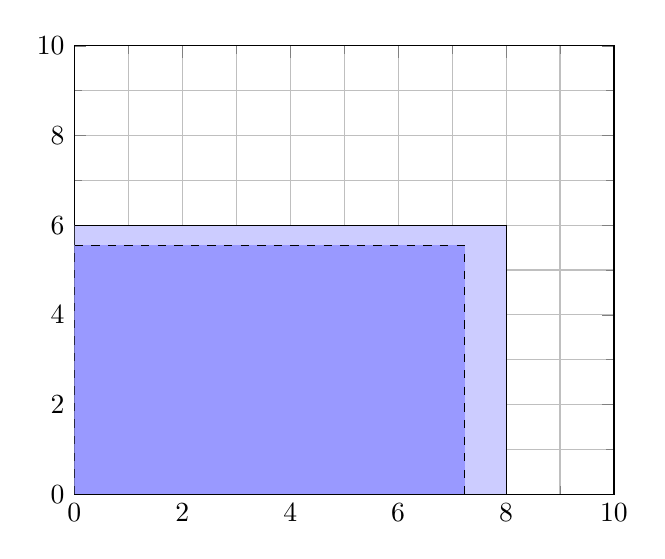
\begin{tikzpicture}
        \begin{axis}[xshift=0.7cm, xmin=0, xmax=10, ymin=0, ymax=10, grid=both, minor tick num=1]
            \filldraw[draw=black,fill=blue!20] (axis cs:0, 0) rectangle (axis cs:8, 6);
            \filldraw[draw=black,fill=blue!40,dashed] (axis cs:0,0) rectangle (axis cs:7.23, 5.55);
        \end{axis}
    \end{tikzpicture}
    \caption{Discretization of an item for the 2DKP covering model.}
    \label{fig:2DKP covering discretization example}
\end{figure}

In the covering model, we introduce binary matrix $A \in \mathbb{R}^{n \times 2 \times W \times H}$. If item $k$ can be placed at cell $(i,j)$ with rotation $r$ without leaving the boundaries of the container, then $A_{k,i,j,r} = 1$. Otherwise, $A_{k,r,i,j} = 0$. By convention,

\begin{align}
    r = 1& \Rightarrow \text{item is not rotated,}\nonumber\\
    r = 2& \Rightarrow \text{item is rotated.}\nonumber
\end{align}

Next, we introduce binary matrix $C \in \mathbb{R}^{n \times 2 \times W \times H \times W \times H}$. If cells $(i',j')$ are covered as a result of item $k$ being placed at cell $(i,j)$ with rotation $r$, then $C_{k,r,i,j,i',j'} = 1$. Otherwise, $C_{k,r,i,j,i',j'} = 0$.

Lastly, we make the decision variables $s_{k,r,i,j}$, since item placement is based on the top-left cell of each item. This is enough to formulate \cref{eq:ip:2DKP covering}.

\begin{subequations}
    \label[ip]{eq:ip:2DKP covering}
    \begin{align}
        \max &\sum_{n,r,i,j \mid A_{n,r,i,j} = 1} v_i s_{k,r,i,j}\\
        \text{s. t.} &\sum_{k,r,i,j \mid C_{k,r,i,j,i',j'} = 1} s_{k,r,i,j} \leq 1, \quad \forall i' \in \{1,\dots,W\}, \, j' \in \{1,\dots,H\},\\
        &\sum_{r,i,j \mid A_{k,r,i,j} = 1} s_{k,r,i,j} \leq 1, \quad \forall k \in \{1,\dots,n\}\\
        &s_{k,r,i,j} \in \{0,1\}.
    \end{align}
\end{subequations}

We have also written an \href{https://github.com/phcentenaro7/IC-Knapsack/blob/957b87062cb846a6e30e7c0a9246ad8b6f7bd189/Knapsack/Kalvelagen/jump_2dknapsack_covering.jl}{implementation} of this model. The model we implemented is the one presented by \textcite{KALVELAGEN2021}, which is more memory-efficient than \cref{eq:ip:2DKP covering}, since it groups items of the same type together in the matrices.

\begin{example}
    
\end{example}